\subsection{Tables and Venn diagrams for single and shared SNPs}

MultiGWAS provides tabular and graphic views to report the best-ranked and significant SNPs identified by the four GWAS packages in an integrative way (see Figure \ref{fig:Table-Shared-SNPs}). Both \emph{p-values} and significance levels have been scaled as $-log_{10}(\mathB{p-value})$ to give high scores to the best statistically evaluated SNPs.

First, best-ranked SNPs correspond to the top-scored \emph{N} SNPs, whether they were assessed significant or not by its package, and with\emph{
N} defined by the user in the configuration file. These SNPs appears in both a SNPs table (Figure \ref{fig:Table-Shared-SNPs}.a), and in
a Venn diagram (Figure \ref{fig:Table-Shared-SNPs}.b). The table lists them by package and sorts by decreasing score, whereas the Venn diagram emphasizes if they were best-ranked either in a single package or in several at once (shared). 

Second, the significant SNPs correspond to the ones valued statistically significant by each package. They appear in a Venn diagram (Figure \ref{fig:Table-Shared-SNPs}.c), and in the SNPs table, marked with significance TRUE (T) in the table of the Figure \ref{fig:Table-Shared-SNPs}.a.

\begin{figure}[H]
\begin{centering}
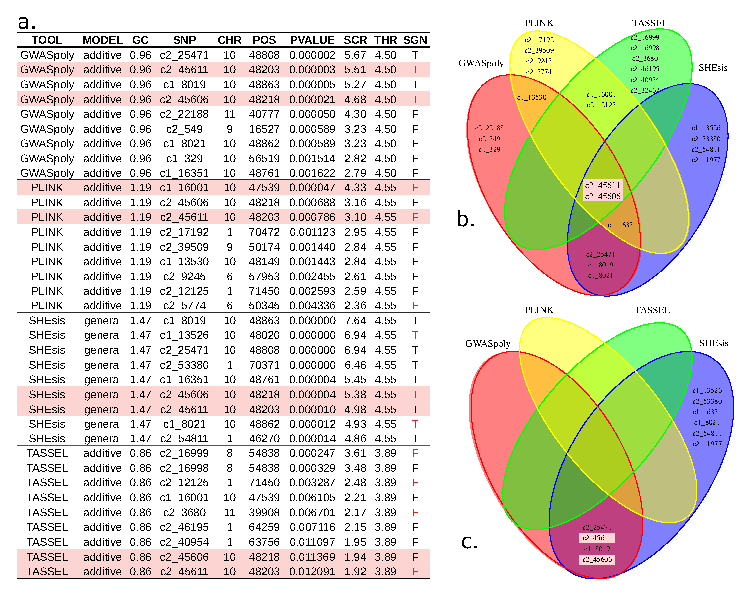
\includegraphics{images/paper-table-venn-best}
\par\end{centering}
\caption{\textbf{Shared SNPs Views. } Tabular and graphical views of SNP associations identified by one or more GWAS packages (shared SNPs). SNPs identified by all packages are marker with red background in all figures. \textbf{(a)} Table with details of the N=9 best-ranked SNPs from each GWAS package. Each row corresponds to a single SNP, and the nine columns are tool name,
the model used by the tool, genomic control factor (inflation factor), SNP name, chromosome, position in the genome, \emph{p-value}, score
as $-log_{10}(\mathB{p-value})$, significance threshold as $-log_{10}(\alpha/m)$ where $\alpha$ is the significance level, and $m$ is the number of
tested markers, and significance as true (T) or false (F) whether score > threshold or not. \textbf{(b)} Venn diagram of the N=9 best-ranked SNPs. SNPs identified by all packages are in the central intersection. Other SNPs identified by more than one packages are in both upper central and lower central intersections. \textbf{(c)} Venn diagram of the significant SNPs (score > threshold). \label{fig:Table-Shared-SNPs}}
\end{figure}

